\documentclass[12pt,letterpaper]{article}
\usepackage{graphicx,textcomp}
\usepackage{natbib}
\usepackage{setspace}
\usepackage{fullpage}
\usepackage{color}
\usepackage[reqno]{amsmath}
\usepackage{amsthm}
\usepackage{fancyvrb}
\usepackage{amssymb,enumerate}
\usepackage[all]{xy}
\usepackage{endnotes}
\usepackage{lscape}
\newtheorem{com}{Comment}
\usepackage{float}
\usepackage{hyperref}
\newtheorem{lem} {Lemma}
\newtheorem{prop}{Proposition}
\newtheorem{thm}{Theorem}
\newtheorem{defn}{Definition}
\newtheorem{cor}{Corollary}
\newtheorem{obs}{Observation}
\usepackage[compact]{titlesec}
\usepackage{dcolumn}
\usepackage{tikz}
\usetikzlibrary{arrows}
\usepackage{multirow}
\usepackage{subcaption}
\usepackage{xcolor}
\newcolumntype{.}{D{.}{.}{-1}}
\newcolumntype{d}[1]{D{.}{.}{#1}}
\definecolor{light-gray}{gray}{0.65}
\usepackage{url}
\usepackage{listings}
\usepackage{color}
\definecolor{codegreen}{rgb}{0,0.6,0}
\definecolor{codegray}{rgb}{0.5,0.5,0.5}
\definecolor{codepurple}{rgb}{0.58,0,0.82}
\definecolor{backcolour}{rgb}{0.95,0.95,0.92}

\lstdefinestyle{mystyle}{
	backgroundcolor=\color{backcolour},   
	commentstyle=\color{codegreen},
	keywordstyle=\color{magenta},
	numberstyle=\tiny\color{codegray},
	stringstyle=\color{codepurple},
	basicstyle=\footnotesize,
	breakatwhitespace=false,         
	breaklines=true,                 
	captionpos=b,                    
	keepspaces=true,                 
	numbers=left,                    
	numbersep=5pt,                  
	showspaces=false,                
	showstringspaces=false,
	showtabs=false,                  
	tabsize=2
}
\lstset{style=mystyle}
\newcommand{\Sref}[1]{Section~\ref{#1}}

\title{ Price House Group Project}
\date{November 9th, 2022}
\author{Group A}

\begin{document}
	\maketitle
	
\section{House Price Models}

\begin{verbatim}
	\lstinputlisting[language=R, firstline=20, lastline=25]{House_Price_Project.R}}
\end{verbatim}
	
% Table created by stargazer v.5.2.3 by Marek Hlavac, Social Policy Institute. E-mail: marek.hlavac at gmail.com% Date and time: Thu, Nov 10, 2022 - 08:58:18
\begin{table}[!htbp] \centering   \caption{Summary of first Model}   \label{} \begin{tabular}{@{\extracolsep{5pt}}lc} \\[-1.8ex]\hline \hline \\[-1.8ex]  & \multicolumn{1}{c}{\textit{Dependent variable:}} \\ \cline{2-2} \\[-1.8ex] & SalePrice \\ \hline \\[-1.8ex]  AdjSalePrice & 0.884$^{***}$ \\   & (0.001) \\   & \\  Constant & 7,868.677$^{***}$ \\   & (727.608) \\   & \\ \hline \\[-1.8ex] Observations & 20,340 \\ R$^{2}$ & 0.971 \\ Adjusted R$^{2}$ & 0.971 \\ Residual Std. Error & 58,683.330 (df = 20338) \\ F Statistic & 692,748.400$^{***}$ (df = 1; 20338) \\ \hline \hline \\[-1.8ex] \textit{Note:}  & \multicolumn{1}{r}{$^{*}$p$<$0.1; $^{**}$p$<$0.05; $^{***}$p$<$0.01} \\ 
\end{tabular} 
\end{table} 

\begin{verbatim}
	
\lstinputlisting[language=R, firstline=05, lastline=25]{House_Price_Project.R}  

\end{verbatim}

\vspace{.25cm}
\noindent With our figure saved, we just need to render it in our .tex file, which we can do using the \texttt{figure} environment:


\begin{verbatim}
	\begin{figure}[h!]\centering
		\caption{\footnotesize Plot for Sales Price}
		\label{fig:plot_1}
		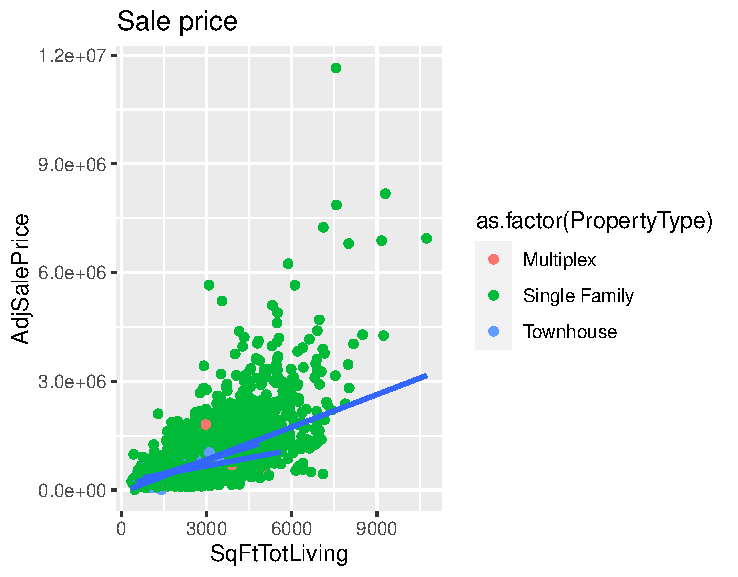
\includegraphics[width=.85\textwidth]{saleprice.pdf}
	\end{figure}
\end{verbatim}

\end{document}

